\documentclass{extbook}[14pt]
\usepackage{multicol, enumerate, enumitem, hyperref, color, soul, setspace, parskip, fancyhdr, amssymb, amsthm, amsmath, bbm, latexsym, units, mathtools}
\everymath{\displaystyle}
\usepackage[headsep=0.5cm,headheight=0cm, left=1 in,right= 1 in,top= 1 in,bottom= 1 in]{geometry}
\usepackage{dashrule}  % Package to use the command below to create lines between items
\newcommand{\litem}[1]{\item #1

\rule{\textwidth}{0.4pt}}
\pagestyle{fancy}
\lhead{}
\chead{Answer Key for Progress Quiz 4 Version A}
\rhead{}
\lfoot{4378-7085}
\cfoot{}
\rfoot{Fall 2020}
\begin{document}
\textbf{This key should allow you to understand why you choose the option you did (beyond just getting a question right or wrong). \href{https://xronos.clas.ufl.edu/mac1105spring2020/courseDescriptionAndMisc/Exams/LearningFromResults}{More instructions on how to use this key can be found here}.}

\textbf{If you have a suggestion to make the keys better, \href{https://forms.gle/CZkbZmPbC9XALEE88}{please fill out the short survey here}.}

\textit{Note: This key is auto-generated and may contain issues and/or errors. The keys are reviewed after each exam to ensure grading is done accurately. If there are issues (like duplicate options), they are noted in the offline gradebook. The keys are a work-in-progress to give students as many resources to improve as possible.}

\rule{\textwidth}{0.4pt}

\begin{enumerate}\litem{
Choose the graph of the equation below.
\[ f(x) = \frac{-1}{(x + 1)^2} - 3 \]
The solution is the graph below, which is option B.
\begin{center}
    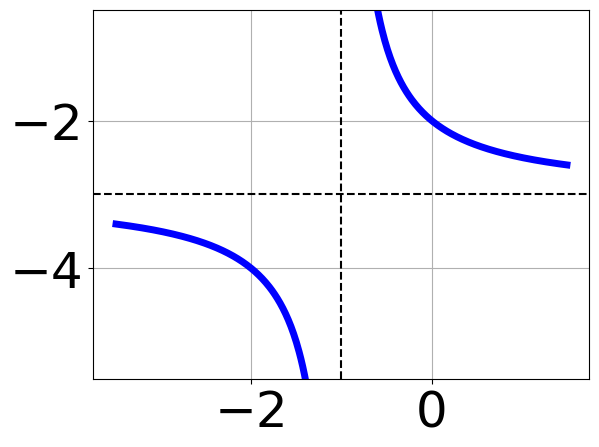
\includegraphics[width=0.3\textwidth]{../Figures/rationalEquationToGraphCopyBA.png}
\end{center}\begin{enumerate}[label=\Alph*.]
\begin{multicols}{2}
\item 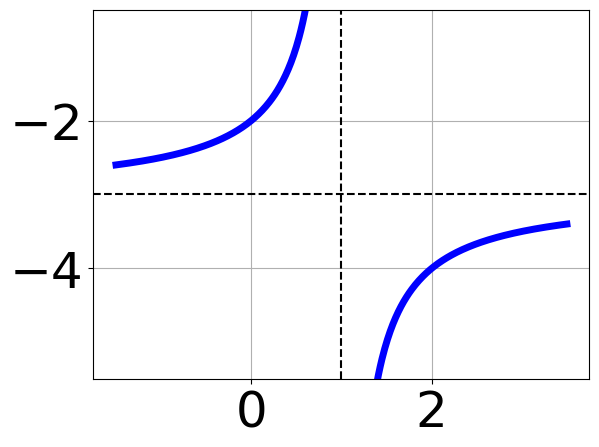
\includegraphics[width = 0.3\textwidth]{../Figures/rationalEquationToGraphCopyAA.png}
\item 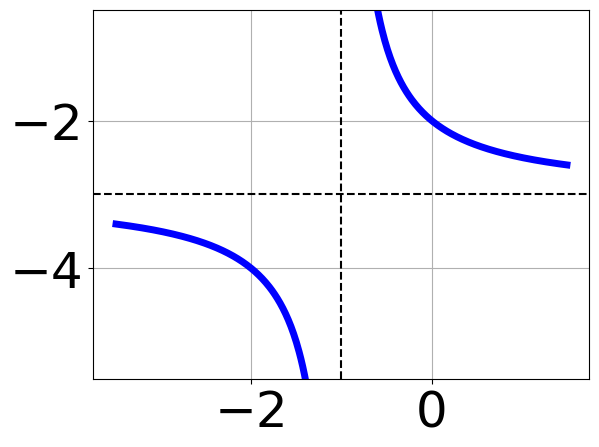
\includegraphics[width = 0.3\textwidth]{../Figures/rationalEquationToGraphCopyBA.png}
\item 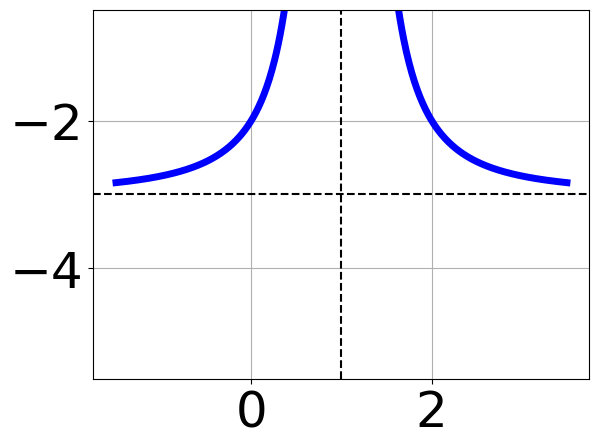
\includegraphics[width = 0.3\textwidth]{../Figures/rationalEquationToGraphCopyCA.png}
\item 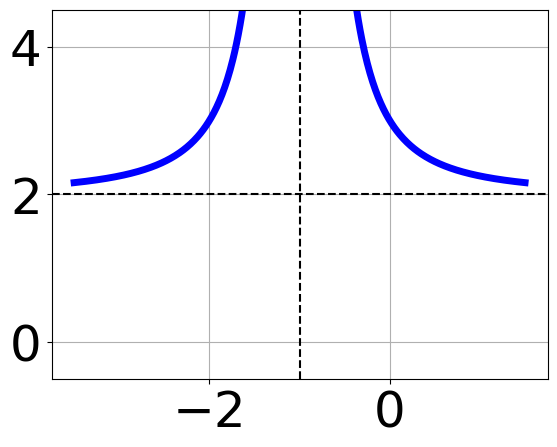
\includegraphics[width = 0.3\textwidth]{../Figures/rationalEquationToGraphCopyDA.png}
\end{multicols}\item None of the above.\end{enumerate}
\textbf{General Comment:} Remember that the general form of a basic rational equation is $ f(x) = \frac{a}{(x-h)^n} + k$, where $a$ is the leading coefficient (and in this case, we assume is either $1$ or $-1$), $n$ is the degree (in this case, either $1$ or $2$), and $(h, k)$ is the intersection of the asymptotes.
}
\litem{
Choose the equation of the function graphed below.

\begin{center}
    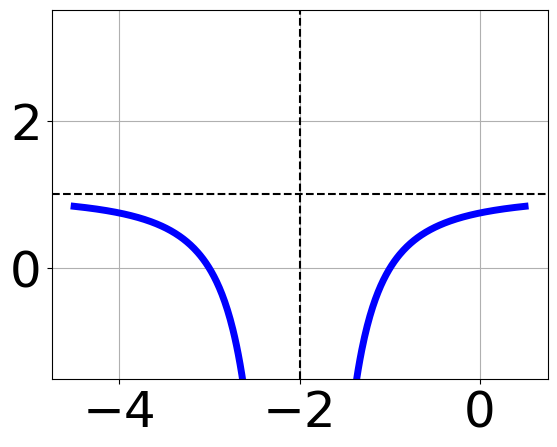
\includegraphics[width=0.5\textwidth]{../Figures/rationalGraphToEquationCopyA.png}
\end{center}



The solution is \( f(x) = \frac{-1}{(x + 2)^2} + 3 \), which is option C.\begin{enumerate}[label=\Alph*.]
\item \( f(x) = \frac{1}{x - 2} + 3 \)

Corresponds to thinking the graph was a shifted version of $\frac{1}{x}$, using the general form $f(x) = \frac{a}{(x+h)^2}+k$, and the opposite leading coefficient.
\item \( f(x) = \frac{-1}{x + 2} + 3 \)

Corresponds to thinking the graph was a shifted version of $\frac{1}{x}$.
\item \( f(x) = \frac{-1}{(x + 2)^2} + 3 \)

This is the correct option.
\item \( f(x) = \frac{1}{(x - 2)^2} + 3 \)

Corresponds to using the general form $f(x) = \frac{a}{(x+h)^2}+k$ and the opposite leading coefficient.
\item \( \text{None of the above} \)

This corresponds to believing the vertex of the graph was not correct.
\end{enumerate}

\textbf{General Comment:} Remember that the general form of a basic rational equation is $ f(x) = \frac{a}{(x-h)^n} + k$, where $a$ is the leading coefficient (and in this case, we assume is either $1$ or $-1$), $n$ is the degree (in this case, either $1$ or $2$), and $(h, k)$ is the intersection of the asymptotes.
}
\litem{
Choose the equation of the function graphed below.

\begin{center}
    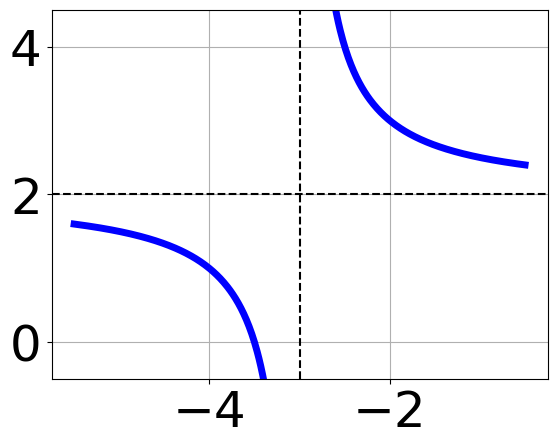
\includegraphics[width=0.5\textwidth]{../Figures/rationalGraphToEquationA.png}
\end{center}



The solution is \( f(x) = \frac{-1}{x - 3} + 2 \), which is option D.\begin{enumerate}[label=\Alph*.]
\item \( f(x) = \frac{-1}{(x - 3)^2} + 2 \)

Corresponds to thinking the graph was a shifted version of $\frac{1}{x^2}$.
\item \( f(x) = \frac{1}{(x + 3)^2} + 2 \)

Corresponds to thinking the graph was a shifted version of $\frac{1}{x^2}$, using the general form $f(x) = \frac{a}{x+h}+k$, and the opposite leading coefficient.
\item \( f(x) = \frac{1}{x + 3} + 2 \)

Corresponds to using the general form $f(x) = \frac{a}{x+h}+k$ and the opposite leading coefficient.
\item \( f(x) = \frac{-1}{x - 3} + 2 \)

This is the correct option.
\item \( \text{None of the above} \)

This corresponds to believing the vertex of the graph was not correct.
\end{enumerate}

\textbf{General Comment:} Remember that the general form of a basic rational equation is $ f(x) = \frac{a}{(x-h)^n} + k$, where $a$ is the leading coefficient (and in this case, we assume is either $1$ or $-1$), $n$ is the degree (in this case, either $1$ or $2$), and $(h, k)$ is the intersection of the asymptotes.
}
\litem{
Solve the rational equation below. Then, choose the interval(s) that the solution(s) belongs to.
\[ \frac{54}{48x + 24} + 1 = \frac{54}{48x + 24} \]
The solution is \( \text{all solutions are invalid or lead to complex values in the equation.} \), which is option A.\begin{enumerate}[label=\Alph*.]
\item \( \text{All solutions lead to invalid or complex values in the equation.} \)

*$x = -0.500$ leads to dividing by 0 in the original equation and thus is not a valid solution, which is the correct option.
\item \( x \in [-0.5,1.5] \)

$x = -0.500$, which corresponds to not checking if this value leads to dividing by 0 in the original equation and thus is not a valid solution.
\item \( x \in [0.09,0.75] \)

$x = 0.500$, which corresponds to not distributing the factor $48x + 24$ correctly when trying to eliminate the fraction.
\item \( x_1 \in [-0.59, 0.21] \text{ and } x_2 \in [0,1.1] \)

$x = -0.500 \text{ and } x = 0.500$, which corresponds to getting the correct solution and believing there should be a second solution to the equation.
\item \( x_1 \in [-0.59, 0.21] \text{ and } x_2 \in [-1.2,-0.1] \)

$x = -0.500 \text{ and } x = -0.500$, which corresponds to getting the correct solution and believing there should be a second solution to the equation.
\end{enumerate}

\textbf{General Comment:} Distractors are different based on the number of solutions. Remember that after solving, we need to make sure our solution does not make the original equation divide by zero!
}
\litem{
Choose the graph of the equation below.
\[ f(x) = \frac{-1}{(x + 1)^2} + 1 \]
The solution is the graph below, which is option E.
\begin{center}
    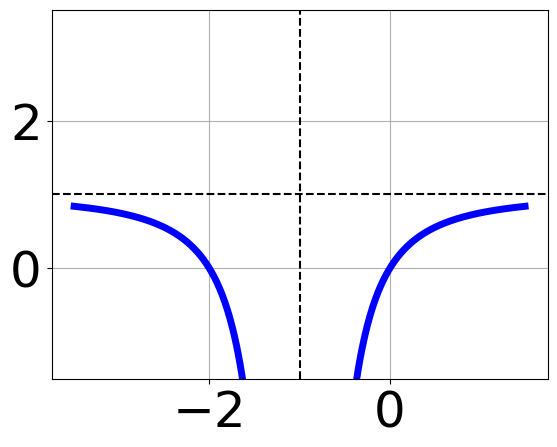
\includegraphics[width=0.3\textwidth]{../Figures/rationalEquationToGraphEA.png}
\end{center}\begin{enumerate}[label=\Alph*.]
\begin{multicols}{2}
\item 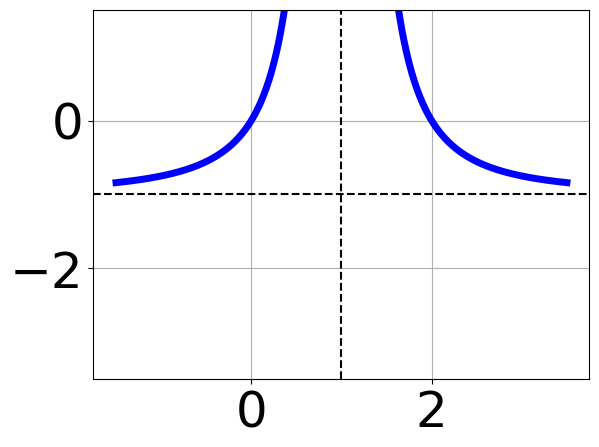
\includegraphics[width = 0.3\textwidth]{../Figures/rationalEquationToGraphAA.png}
\item 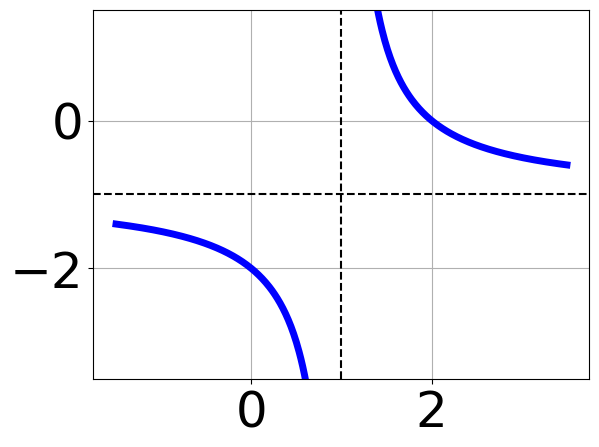
\includegraphics[width = 0.3\textwidth]{../Figures/rationalEquationToGraphBA.png}
\item 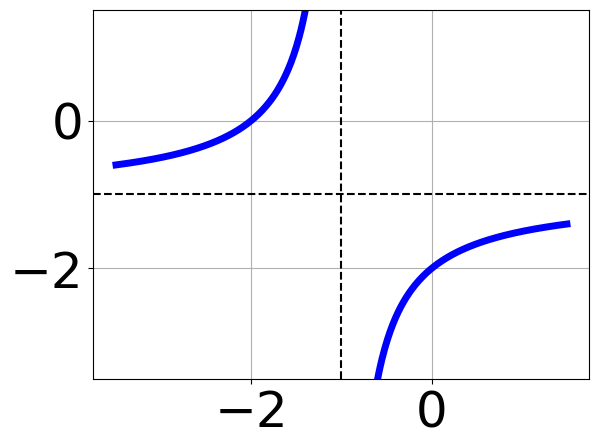
\includegraphics[width = 0.3\textwidth]{../Figures/rationalEquationToGraphCA.png}
\item 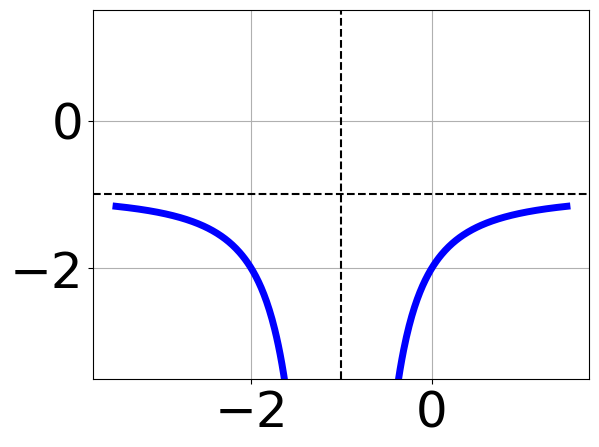
\includegraphics[width = 0.3\textwidth]{../Figures/rationalEquationToGraphDA.png}
\end{multicols}\item None of the above.\end{enumerate}
\textbf{General Comment:} Remember that the general form of a basic rational equation is $ f(x) = \frac{a}{(x-h)^n} + k$, where $a$ is the leading coefficient (and in this case, we assume is either $1$ or $-1$), $n$ is the degree (in this case, either $1$ or $2$), and $(h, k)$ is the intersection of the asymptotes.
}
\litem{
Solve the rational equation below. Then, choose the interval(s) that the solution(s) belongs to.
\[ \frac{-2x}{3x -3} + \frac{-2x^{2}}{6x^{2} -24 x + 18} = \frac{-7}{2x -6} \]
The solution is \( \text{There are two solutions: } x = 0.734 \text{ and } x = 4.766 \), which is option D.\begin{enumerate}[label=\Alph*.]
\item \( x \in [3.4,7.5] \)


\item \( \text{All solutions lead to invalid or complex values in the equation.} \)


\item \( x \in [0.8,3.4] \)


\item \( x_1 \in [-1, 0.9] \text{ and } x_2 \in [3.77,6.77] \)

* $x = 0.734 \text{ and } x = 4.766$, which is the correct option.
\item \( x_1 \in [-1, 0.9] \text{ and } x_2 \in [-3,3] \)


\end{enumerate}

\textbf{General Comment:} Distractors are different based on the number of solutions. Remember that after solving, we need to make sure our solution does not make the original equation divide by zero!
}
\litem{
Determine the domain of the function below.
\[ f(x) = \frac{6}{16x^{2} -12 x -18} \]
The solution is \( \text{All Real numbers except } x = -0.750 \text{ and } x = 1.500. \), which is option D.\begin{enumerate}[label=\Alph*.]
\item \( \text{All Real numbers except } x = a, \text{ where } a \in [-13, -10] \)

All Real numbers except $x = -12.000$, which corresponds to removing a distractor value from the denominator.
\item \( \text{All Real numbers except } x = a, \text{ where } a \in [-0.75, 1.25] \)

All Real numbers except $x = -0.750$, which corresponds to removing only 1 value from the denominator.
\item \( \text{All Real numbers except } x = a \text{ and } x = b, \text{ where } a \in [-13, -10] \text{ and } b \in [23, 27] \)

All Real numbers except $x = -12.000$ and $x = 24.000$, which corresponds to not factoring the denominator correctly.
\item \( \text{All Real numbers except } x = a \text{ and } x = b, \text{ where } a \in [-0.75, 1.25] \text{ and } b \in [1.5, 8.5] \)

All Real numbers except $x = -0.750$ and $x = 1.500$, which is the correct option.
\item \( \text{All Real numbers.} \)

This corresponds to thinking the denominator has complex roots or that rational functions have a domain of all Real numbers.
\end{enumerate}

\textbf{General Comment:} Recall that dividing by zero is not a real number. Therefore the domain is all real numbers \textbf{except} those that make the denominator 0.
}
\litem{
Solve the rational equation below. Then, choose the interval(s) that the solution(s) belongs to.
\[ \frac{7x}{5x + 2} + \frac{-4x^{2}}{-10x^{2} +6 x + 4} = \frac{-3}{-2x + 2} \]
The solution is \( \text{There are two solutions: } x = -0.186 \text{ and } x = 1.797 \), which is option C.\begin{enumerate}[label=\Alph*.]
\item \( x_1 \in [-1.45, 0.43] \text{ and } x_2 \in [-2.3,0.4] \)


\item \( x \in [1.24,2.03] \)


\item \( x_1 \in [-1.45, 0.43] \text{ and } x_2 \in [0.1,2] \)

* $x = -0.186 \text{ and } x = 1.797$, which is the correct option.
\item \( x \in [0.9,1.67] \)


\item \( \text{All solutions lead to invalid or complex values in the equation.} \)


\end{enumerate}

\textbf{General Comment:} Distractors are different based on the number of solutions. Remember that after solving, we need to make sure our solution does not make the original equation divide by zero!
}
\litem{
Determine the domain of the function below.
\[ f(x) = \frac{3}{15x^{2} -3 x -18} \]
The solution is \( \text{All Real numbers except } x = -1.000 \text{ and } x = 1.200. \), which is option D.\begin{enumerate}[label=\Alph*.]
\item \( \text{All Real numbers except } x = a, \text{ where } a \in [-1, 0] \)

All Real numbers except $x = -1.000$, which corresponds to removing only 1 value from the denominator.
\item \( \text{All Real numbers except } x = a \text{ and } x = b, \text{ where } a \in [-11, -4] \text{ and } b \in [30, 34] \)

All Real numbers except $x = -9.000$ and $x = 30.000$, which corresponds to not factoring the denominator correctly.
\item \( \text{All Real numbers.} \)

This corresponds to thinking the denominator has complex roots or that rational functions have a domain of all Real numbers.
\item \( \text{All Real numbers except } x = a \text{ and } x = b, \text{ where } a \in [-1, 0] \text{ and } b \in [-0.8, 4.2] \)

All Real numbers except $x = -1.000$ and $x = 1.200$, which is the correct option.
\item \( \text{All Real numbers except } x = a, \text{ where } a \in [-11, -4] \)

All Real numbers except $x = -9.000$, which corresponds to removing a distractor value from the denominator.
\end{enumerate}

\textbf{General Comment:} Recall that dividing by zero is not a real number. Therefore the domain is all real numbers \textbf{except} those that make the denominator 0.
}
\litem{
Solve the rational equation below. Then, choose the interval(s) that the solution(s) belongs to.
\[ \frac{-3}{5x -4} + -9 = \frac{-3}{-25x + 20} \]
The solution is \( x = 0.720 \), which is option A.\begin{enumerate}[label=\Alph*.]
\item \( x \in [0.72,1.72] \)

* $x = 0.720$, which is the correct option.
\item \( x_1 \in [0.72, 2.72] \text{ and } x_2 \in [0.79,0.96] \)

$x = 0.720 \text{ and } x = 0.800$, which corresponds to getting the correct solution and believing there should be a second solution to the equation.
\item \( x_1 \in [-0.88, 0.12] \text{ and } x_2 \in [0.62,0.73] \)

$x = -0.880 \text{ and } x = 0.720$, which corresponds to getting the correct solution and believing there should be a second solution to the equation.
\item \( \text{All solutions lead to invalid or complex values in the equation.} \)

This corresponds to thinking $x = 0.720$ leads to dividing by zero in the original equation, which it does not.
\item \( x \in [-0.88,0.12] \)

$x = -0.880$, which corresponds to not distributing the factor $5x -4$ correctly when trying to eliminate the fraction.
\end{enumerate}

\textbf{General Comment:} Distractors are different based on the number of solutions. Remember that after solving, we need to make sure our solution does not make the original equation divide by zero!
}
\end{enumerate}

\end{document}